\documentclass{article}
\usepackage[utf8]{inputenc}
\usepackage{amsmath}
\usepackage{amssymb}
\usepackage{graphicx}

\newcommand\xkn{\mathbf{x}^{\left(k+1\right)}}
\newcommand\xk{\mathbf{x}^{\left(k\right)}}
\newcommand\A{\mathbf{A}}
\newcommand\tr{\mathsf{T}}

\begin{document}
\section*{Gauss-Seidel Iteration for a Sparse Linear System of Equations}
Given a \textbf{regular} square matrix $\mathbf{A}\in\mathbb{R}^{n,n}$ and the vector $\mathbf{b} \in \mathbb{R}^{n}, n \in \mathbb{N}$ the \textbf{Gauss-Seidel iteration} $\xkn := \mathbf{\Phi}\left(\xk\right)$ for $\mathbf{\Phi} : \mathbb{R}^{n} \to \mathbb{R}^{n}$ which is defined as
\begin{equation*}
    \left(\xkn\right)_{i} = \left(\A\right)_{i,i}^{-1}\left(\left(\mathbf{b}\right)_{i} - \sum_{j=1}^{i-1}\left(\mathbf{A}\right)_{i,j}\left(\xkn\right)_{j} - \sum_{j=i+1}^{n}\left(\A\right)_{i,j}\left(\xk\right)_{j}\right)\,,\: i=1,2,\dots,n 
\end{equation*}
where the exercise puts importance on the ordering of $i = 1, 2, \dots,n$ and states that the iterates must be computed in this order. 
\subsection*{2-18.a}
The task here is to determine for what square matrices $\mathbf{A}$ and vectors $\mathbf{b}$ the Gauss-Seidel iteration is well-defined. We can see that both sums and also the first term are in range and hence pose no problem. The problematic term however is the term $\left(\A\right)_{i,i}^{-1}$ which means that we divide by $\left(\A\right)_{i,i}$, hence this is not well-defined if we have $\left(\A\right)_{i,i}\neq 0$, which leads to
\begin{equation*}
    \text{The GS-iteration is well-defined if } \left(\A\right)_{i,i} \neq 0\quad \forall \, 1 \leq i \leq n
\end{equation*}
\subsection*{2-18.b}
We are tasked with implementing a function that computes one step of the Gauss-Seidel iteration and returns \verb|false| if it is not well-defined and \verb|true| if it is well-defined. The result should be stored in the argument \verb|x|. For this purpose let us look at an image from the lecture document. \begin{figure}[!hbt]
    \centering
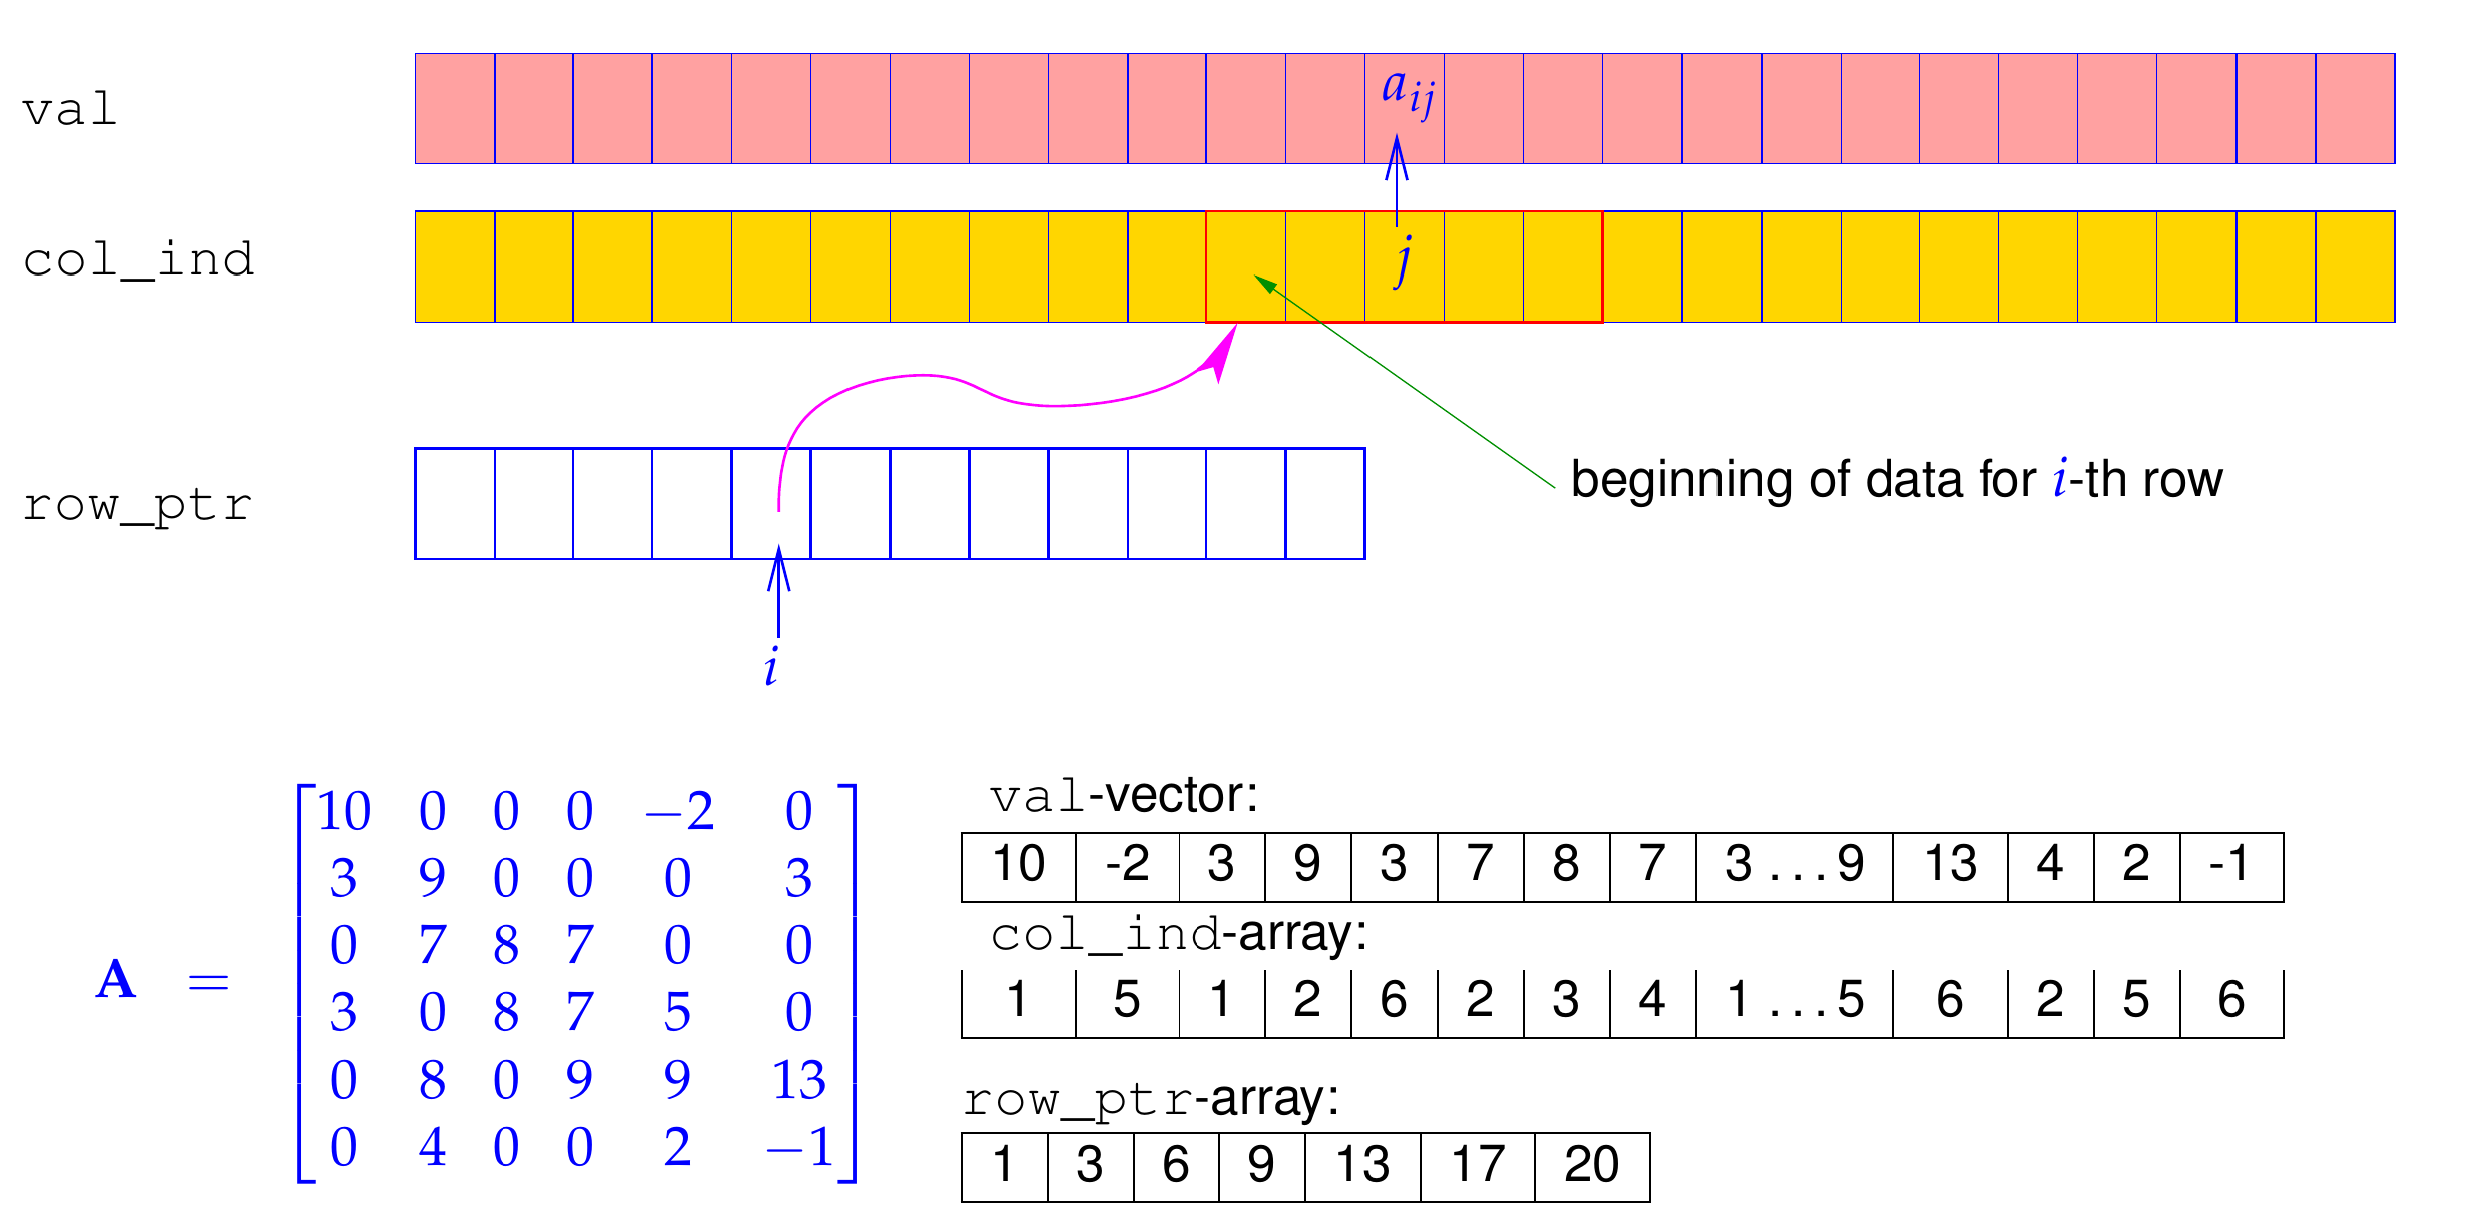
\includegraphics[width=1.0\linewidth]{CRSFormat.png}
\end{figure}
This helps understanding how we can navigate through the matrix. We move row by row, while we find at the corresponding row index $i$ in the \verb|row_ptr| array the start-index for the column positions of the current row in \verb|col_ind.at(i)| and the the end-index at \verb|col_ind.at(i+1)|. We can then use the the direct mapping to get the correct element from the \verb|val| array. This results in the following code
\begin{figure}[!hbt]
    \centering
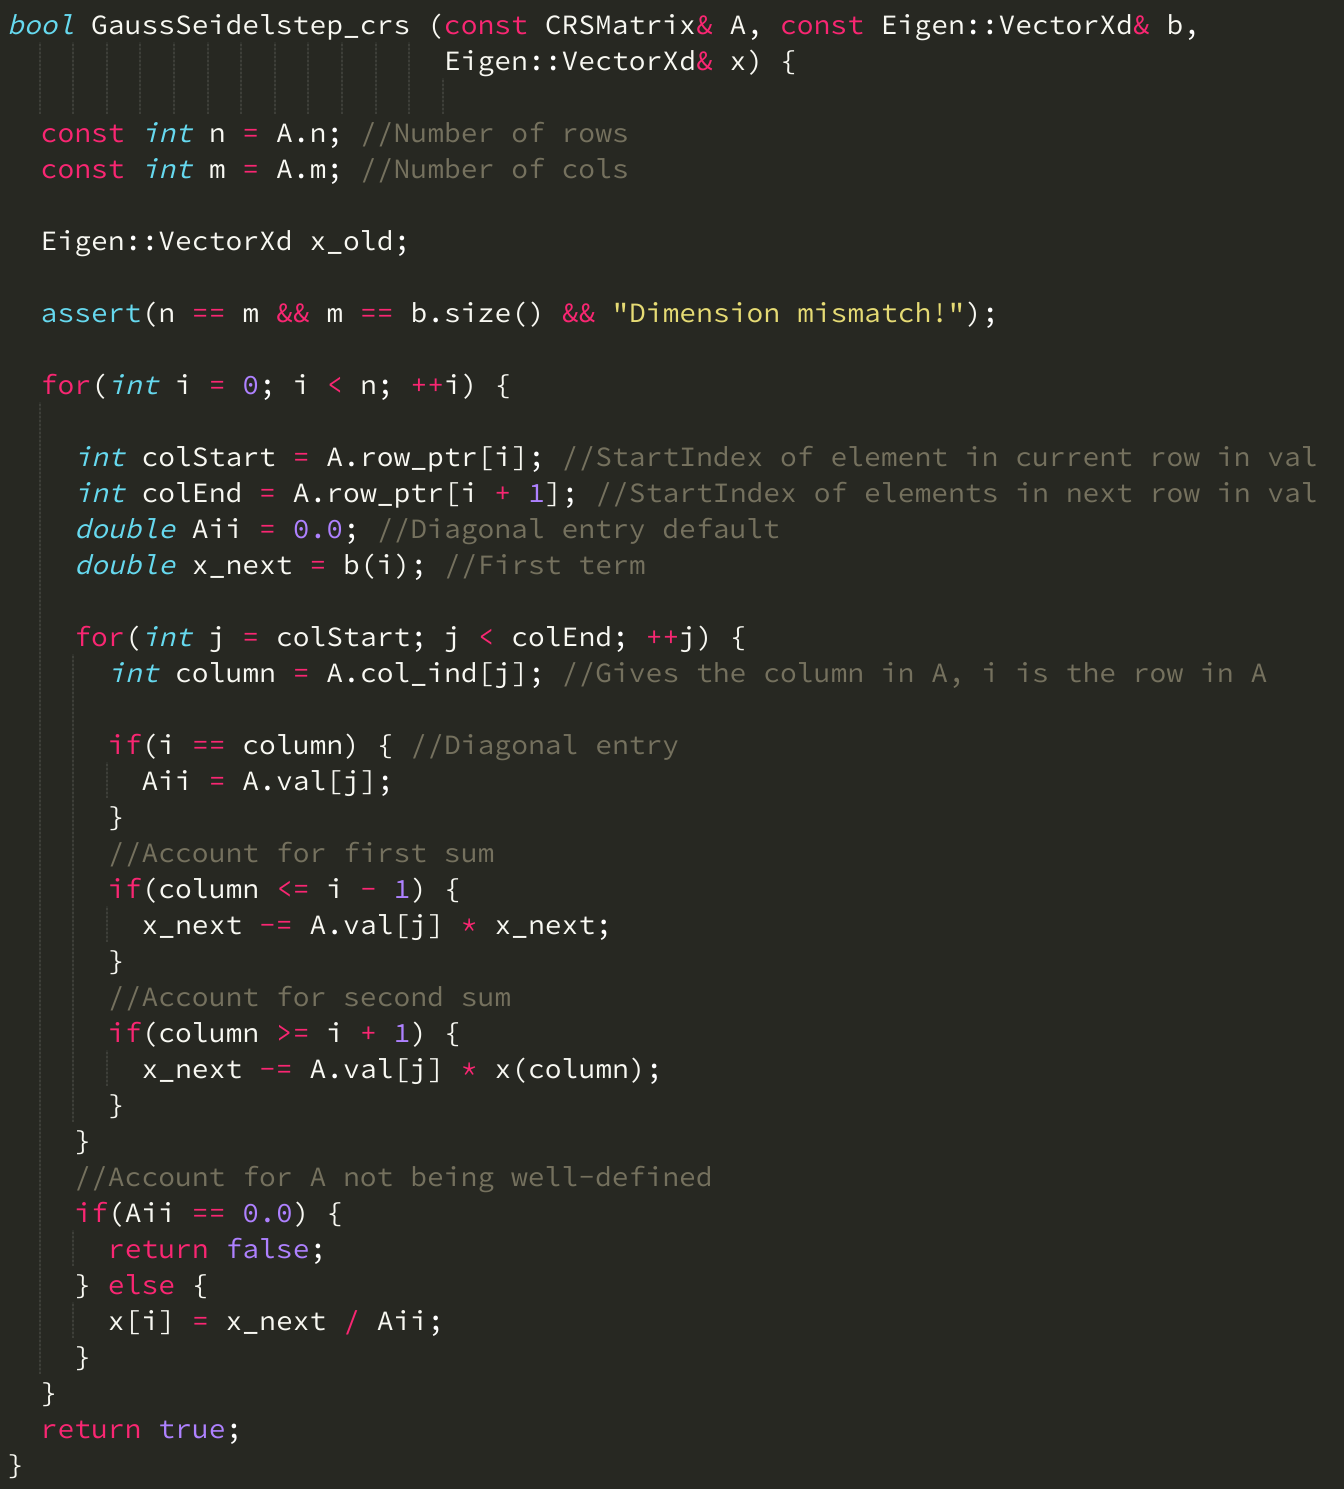
\includegraphics[width=1.0\linewidth]{2-18.b.png}
\end{figure}
\subsection*{2-18.c}
We are given regular $\mathbf{A}\in\mathbb{R}^{n,n}$ and $\mathbf{b}\in \mathbb{R}^{n}$ and assuming that the Gauss-Seidel iteration is well-defined (all diagonal entries of $\mathbf{A}$ are non-zero. We should characterize the set of all \textbf{fixed points} of the Gauss-Seidel iteration by a compact formula. We know that a fixed point of an iteration $\xkn = F\left(\xk\right)$ is a vector $\mathbf{x}^{*}$ such that $\mathbf{x}^{*} = F\left(\mathbf{x}^{*}\right)$. In this example we are hence looking for $\mathbf{x}^{*}$ with $\mathbf{x}^{*} = \mathbf{\Phi}\left(\mathbf{x}^{*}\right)$ Let us put this into the given equation.

\begin{equation*}
   \mathbf{\Phi}\left(\mathbf{x}^{*}\right)_{i} = \left(\A\right)_{i,i}^{-1}\left(\left(\mathbf{b}\right)_{i} - \sum_{j=1}^{i-1}\left(\mathbf{A}\right)_{i,j}\left(\mathbf{\Phi}\left(\mathbf{x}^{*}\right)\right)_{j} - \sum_{j=i+1}^{n}\left(\A\right)_{i,j}\left(\mathbf{x}^{*}\right)_{j}\right)\,,\: i=1,2,\dots,n 
\end{equation*}
It may be helpful to illustrate this for a small example. We define 
\begin{equation*}
    \mathbf{A} = 
    \begin{bmatrix}
    a_{11} & a_{12} & a_{13} \\
    a_{21} & a_{22} & a_{23} \\
    a_{31} & a_{32} & a_{33}
    \end{bmatrix} \quad \text{and} \quad \mathbf{b} = 
    \begin{bmatrix}
        b_{1} \\ b_{2} \\ b_{3}
    \end{bmatrix}
\end{equation*}
We have 
\begin{align*}
    \mathbf{\Phi}\left(\mathbf{x}^{*}\right)_{1} &= \left(\A\right)_{1,1}^{-1}\left(\left(\mathbf{b}\right)_{1} - \sum_{j=1}^{1-1}\left(\mathbf{A}\right)_{1,j}\left(\mathbf{\Phi}\left(\mathbf{x}^{*}\right)\right)_{j} - \sum_{j=1+1}^{3}\left(\A\right)_{1,j}\left(\mathbf{x}^{*}\right)_{j}\right) \\
    &=\left(\A\right)_{1,1}^{-1}\left(\left(\mathbf{b}\right)_{1} - \sum_{j=1}^{0}\left(\mathbf{A}\right)_{1,j}\left(\mathbf{\Phi}\left(\mathbf{x}^{*}\right)\right)_{j} - \sum_{j=2}^{3}\left(\A\right)_{1,j}\left(\mathbf{x}^{*}\right)_{j}\right)  \\
    &=\frac{1}{a_{11}}\left(\left(\mathbf{b}\right)_{1} - \sum_{j=2}^{3}\left(\A\right)_{1,j}\left(\mathbf{x}^{*}\right)_{j}\right) 
\end{align*}
From this it follows that
\begin{equation*}
     a_{11}\cdot \mathbf{\Phi}\left(\mathbf{x}^{*}\right)_{1} = \left(\mathbf{b}\right)_{1} - \sum_{j=2}^{n}\left(\A\right)_{1,j}\left(\mathbf{x}^{*}\right)_{j} = b_{1} - a_{12}x_{2} - a_{13}x_{3}
\end{equation*}
If we force $\mathbf{\Phi}\left(\mathbf{x}^{*}\right)  = \mathbf{x}^{*}$ then we get
\begin{equation}
     a_{11} x^{*}_{1} = b_{1} - a_{12}x^{*}_{2} - a_{13}x^{*}_{3} \implies a_{11} x^{*}_{1}+a_{12}x^{*}_{2} + a_{13}x^{*}_{3} = b_{1}
\end{equation}
Let us look at the next position
\begin{equation*}
   \mathbf{\Phi}\left(\mathbf{x}^{*}\right)_{2} = \left(\A\right)_{2,2}^{-1}\left(\left(\mathbf{b}\right)_{2} - \sum_{j=1}^{2-1}\left(\mathbf{A}\right)_{2,j}\left(\mathbf{\Phi}\left(\mathbf{x}^{*}\right)\right)_{j} - \sum_{j=2+1}^{3}\left(\A\right)_{2,j}\left(\mathbf{x}^{*}\right)_{j}\right) 
\end{equation*}
from this it follows that
\begin{equation}
    a_{22}x^{*}_{2} = b_{2} - a_{21}x^{*}_{1} - a_{23}x^{*}_{3} \implies a_{21}x^{*}_{1} +a_{22}x^{*}_{2} + a_{23}x^{*}_{3} = b_{2}
\end{equation}
and then from the third one we would get
\begin{equation}
    a_{33}x^{*}_{3} = b_{3} - a_{31}x^{*}_{1} - a_{32}x^{*}_{3} \implies a_{31}x^{*}_{1} +a_{32}x^{*}_{2} + a_{33}x^{*}_{3} = b_{3}
\end{equation}

\pagebreak

\noindent We hence find the following (linear) system of equations
\begin{align*}
    a_{11} x^{*}_{1}+a_{12}x^{*}_{2} + a_{13}x^{*}_{3} &= b_{1} \\
    a_{21}x^{*}_{1} +a_{22}x^{*}_{2} + a_{23}x^{*}_{3} &= b_{2} \\
    a_{31}x^{*}_{1} +a_{32}x^{*}_{2} + a_{33}x^{*}_{3} &= b_{3}
\end{align*}

And hence $\mathbf{x}^{*}$ is the solution to the LSE
\begin{equation*}
    \begin{bmatrix}
    a_{11} & a_{12} & a_{13} \\
    a_{21} & a_{22} & a_{23} \\
    a_{31} & a_{32} & a_{33}
    \end{bmatrix} \begin{bmatrix}
        x^{*}_{1} \\x^{*}_{2} \\ x^{*}_{3}
    \end{bmatrix}
    = \begin{bmatrix}
        b_{1} \\ b_{2} \\b_{3}
    \end{bmatrix}
\end{equation*}
And in general we can solve $\mathbf{A}\mathbf{x}^{*} = \mathbf{b}$ to get the fix points and because $\mathbf{A}$ is regular we have that the set of fixed-points is given to us by
\begin{equation*}
    \left\{\mathbf{x}^{*} \in \mathbb{R} \::\: \mathbf{x}^{*} \text{ is fixed point of GS-iteration}\right\} = \left\{\mathbf{A}^{-1}\mathbf{b}\right\}
\end{equation*}
This can also be seen by putting $\mathbf{\Phi}\left(\mathbf{x}^{*}\right)  = \mathbf{x}^{*}$ into the Gauss-Seidel iteration directly. 
\subsection*{2-18.d}
We are tasked with implementing a function \verb|GaussSeidel_iteration| which carries out the Gauss-Seidel iterations for given parameters $\mathbf{A}$,$\mathbf{b}$ and an initial guess $\mathbf{x}^{\left(0\right)}$ passed in \verb|x|. We are supposed to return the result in \verb|x|. We should use a correction-based termination criterion.
\begin{figure}[!hbt]
    \centering
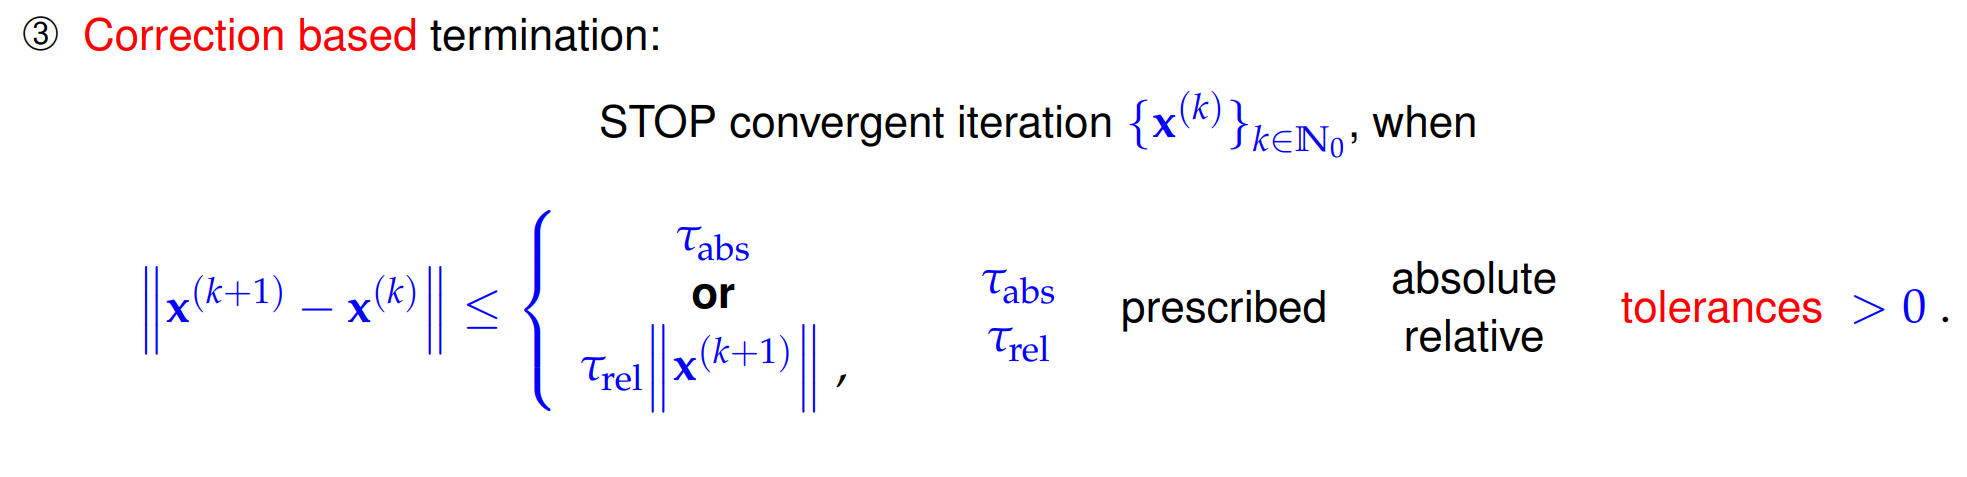
\includegraphics[width=1.0\linewidth]{CorrectionBasedCriterion.png}
\end{figure}
We are given both \verb|atol| and \verb|rtol|, as well as a \verb|maxit| iteration stopping condition, in which case we should return \verb|false|, otherwise we return \verb|true|. 

\pagebreak

\noindent We will use the following piece of code as guide.
\begin{figure}[!hbt]
    \centering
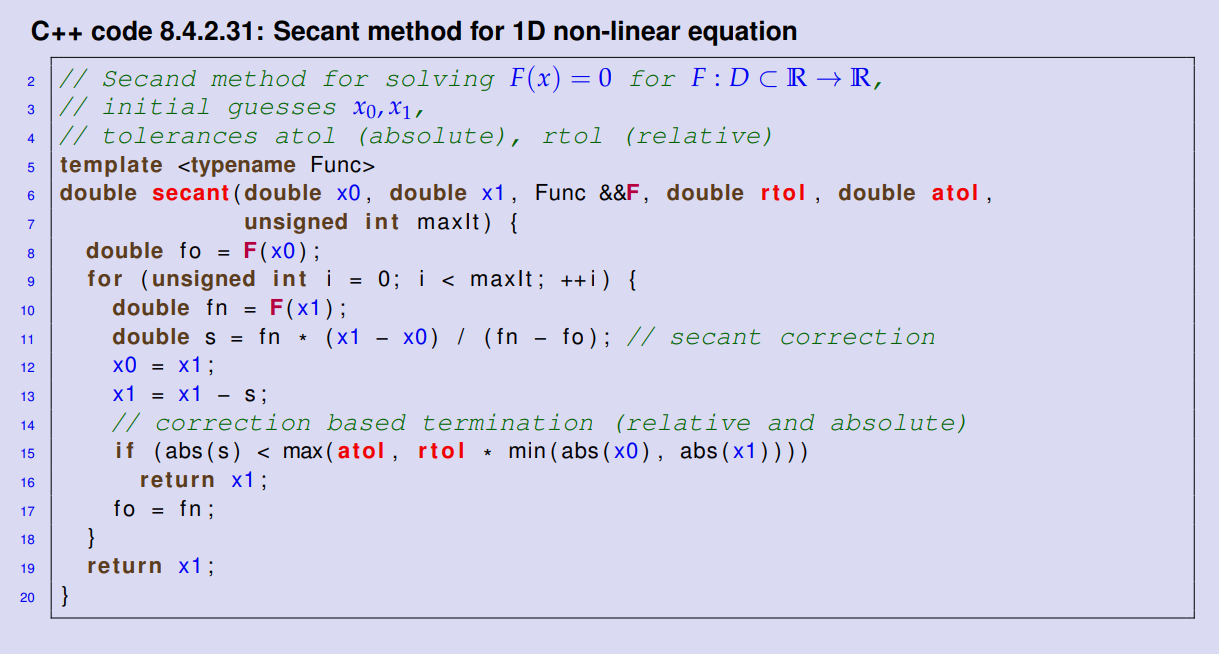
\includegraphics[width=1.0\linewidth]{ExampleCodeCorrBasedFixPoint.png}
\end{figure}

\noindent This gives us the following code.

\begin{figure}[!hbt]
    \centering
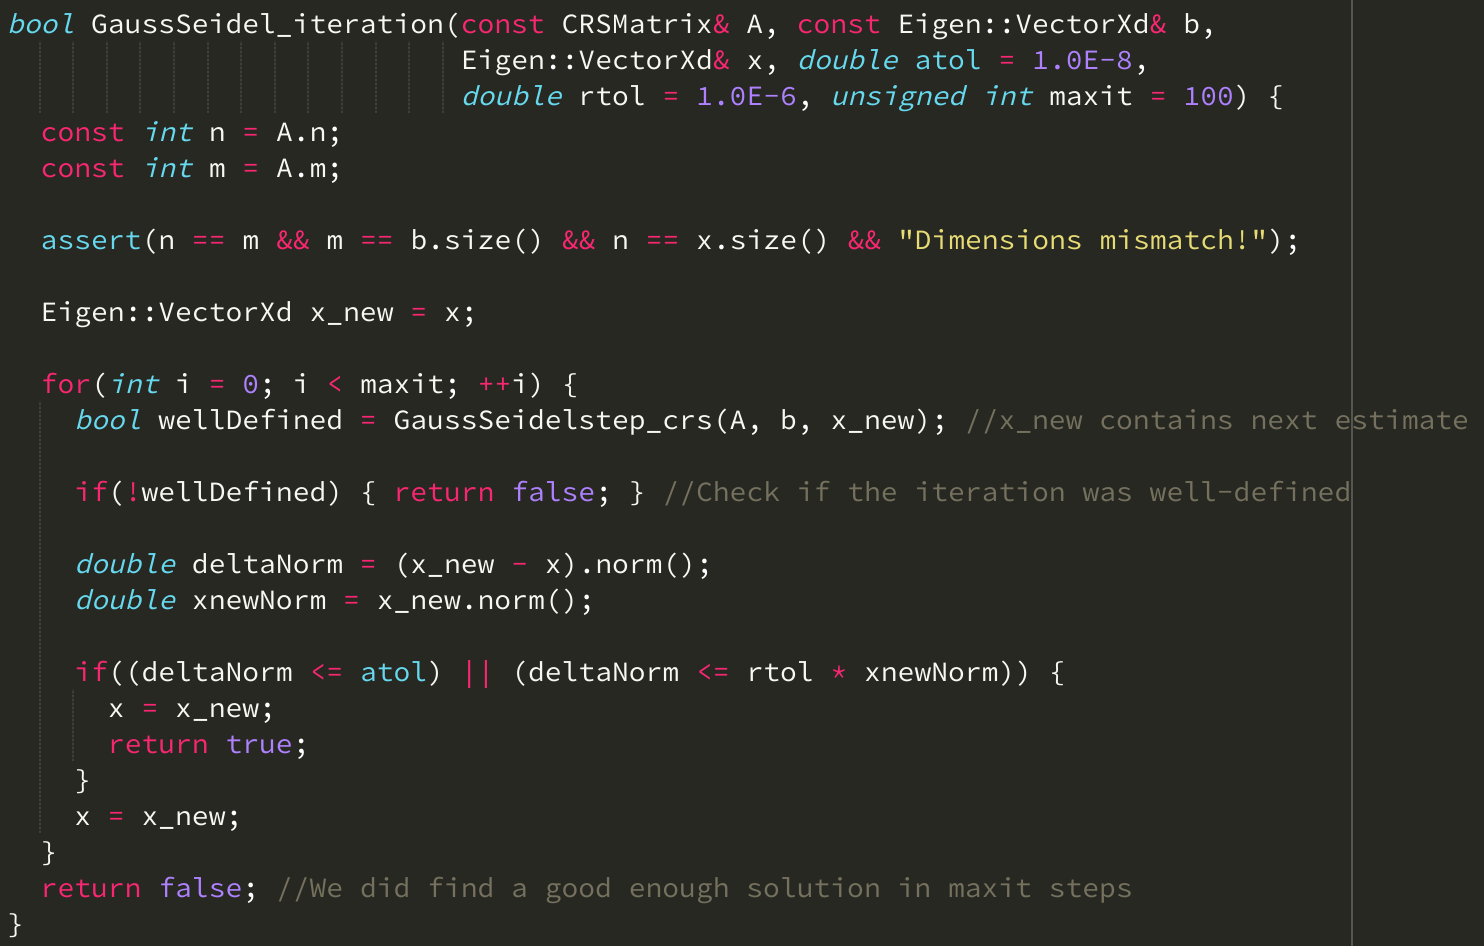
\includegraphics[width=1.0\linewidth]{2-18.d.png}
\end{figure}

\pagebreak

\subsection*{2-18.e}
We are now given the input
\begin{equation*}
    \mathbf{A} = 
    \begin{bmatrix}
        10 & 0 & 0 & 0 & -2 & 0 \\
        3 & 9 & 0 & 0 & 0 & 3 \\
        0 & 2 & 8 & 2 & 0 & 0 \\
        3 & 0 & 1 & 10 & 5 & 0 \\
        0 & 2 & 0 & 3 & 13 & 2 \\
        0 & 4 & 0 & 0 & 2 & 11
    \end{bmatrix}
\end{equation*}
and the inital guess $\mathbf{x}^{\left(0\right)} = \left[1,2,3,4,5,6\right]^{\tr}$. This produces the following numbers.
\begin{figure}[!hbt]
    \centering
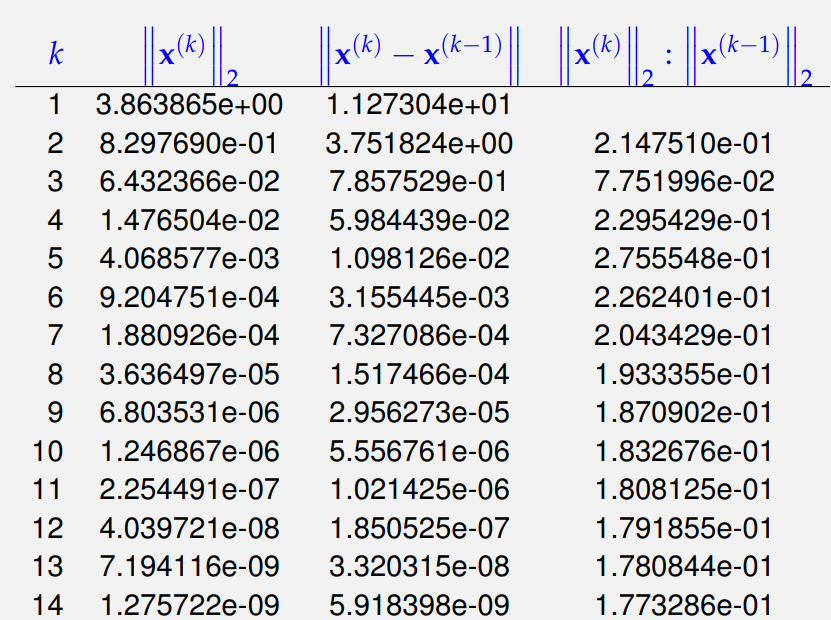
\includegraphics[width=1.0\linewidth]{Stats2-18.e.png}
\end{figure}

\noindent We are now tasked with describing the asymptotic convergence of the iteration for this example. We can see that for $k \to \infty$ we seem to have $\xk \to \mathbf{0}$ because $\left\lVert \xk \right\rVert_{2} \to 0$. We can see that with increasing $k$ the rate of convergence seems to stabilize around the number $0.18$, because we have $\mathbf{x}^{*} = \mathbf{0}$ we also have
\begin{equation*}
    \left\lVert \xkn - \mathbf{x}^{*} \right\rVert_{2} = \left\lVert \xkn \right\rVert_{2} \leq 0.18 \left\lVert \xk - \mathbf{x}^{*} \right\rVert_{2} = 0.18\left\lVert \xk \right\rVert_{2}
\end{equation*}
we can hence conclude a linear convergence with rate $\approx 0.18$. 

\pagebreak

\noindent Some notes on what we did here. We applied the following definition.
\begin{figure}[!hbt]
    \centering
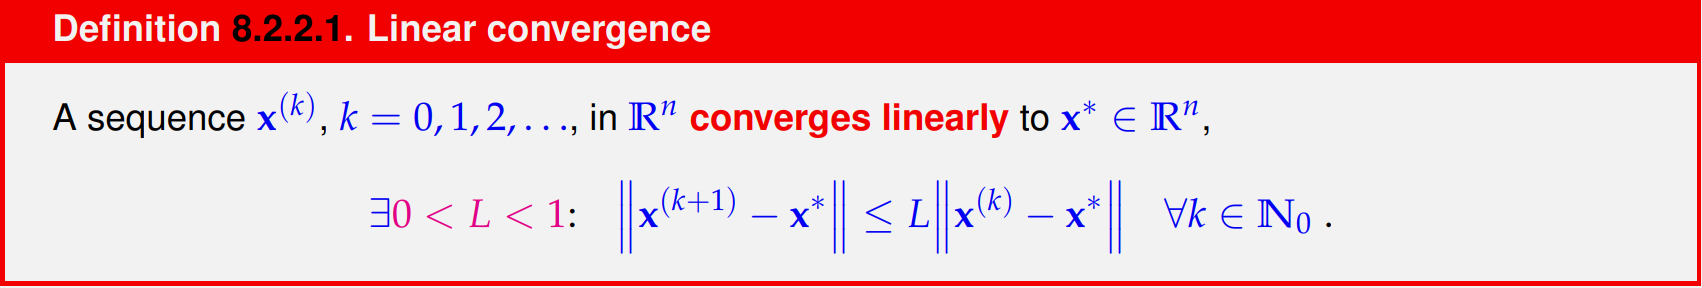
\includegraphics[width=1.0\linewidth]{LinearConvergenceDef.png}
\end{figure}
\end{document}
